%\pgfdeclarelayer{background}
%\pgfdeclarelayer{foreground}
%\pgfsetlayers{background,main,foreground}

\pgfplotsset{
	axis background/.style={fill=none},
	%tick style=mygrey2,
	%tick label style=mygrey2,
	grid=none,
	%xtick pos=left,
	%ytick pos=left,
	tick style={
		major grid style={style=white,line width=1pt},minor grid style=white,
%		major grid style={style=white,line width=1pt},minor grid style=mygrey3,
		%tick align=outside,
	},
	%minor tick num=4,
}

\begin{figure}[b]
	\centering
	\begin{subfigure}[]{0.23\textwidth}
		\centering	
		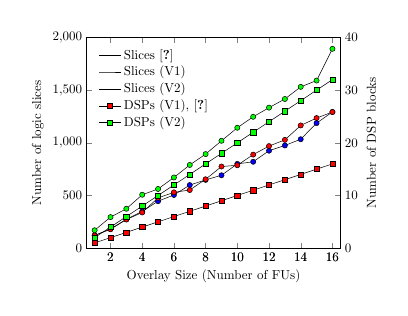
\begin{tikzpicture}[scale = 0.47]
		\begin{axis}[
%		xlabel=Overlay Size (Number of FUs),
		ylabel=Number of logic slices,
		ymax = 2000,
		%ymax = 2500,
		ymin = 0,
		xmax = 16.5,
	    xmin = 0.5,
		legend pos=north west,
		legend cell align={left},
		legend style={draw=none}
		]    
		
		\addplot [mark=*,mark options={fill=blue}] plot coordinates {
			(1,     121)
			(2,     183)
			(3,     274)
			(4,     349)
			(5,     446)
			(6,     505)
			(7,     599)
			(8,     648)
			(9,     692)
			(10,    800)
			(11,    820)
			(12,    925)
			(13,    975)
			(14,    1034)
			(15,    1187)
			(16,    1293)									
		};
		\label{S_olaf}
		\addlegendentry{Slices~\cite{li2016area}}
		
		\addplot [mark=*,mark options={fill=red}] plot coordinates {
			(1,     121)
			(2,     179)
			(3,     272)
			(4,     339)
			(5,     477)
			(6,     530)
			(7,     552)
			(8,     654)
			(9,     775)
			(10,    787)
			(11,    888)
			(12,    969)
			(13,    1028)
			(14,    1165)
			(15,    1235)
			(16,    1292)									
		};
		\label{S_V1}
		\addlegendentry{Slices (V1)}
	
		\addplot [mark=*,mark options={fill=green}] plot coordinates {
			(1,     170)
			(2,     295)
			(3,     374)
			(4,     507)
			(5,     562)
			(6,     671)
			(7,     790)
			(8,     893)
			(9,     1019)
			(10,    1143)
			(11,    1247)
			(12,    1334)
			(13,    1416)
			(14,    1531)
			(15,    1591)
			(16,    1892)			
		};
		\label{S_V2}
		\addlegendentry{Slices (V2)} 
%		\legend{Slices~\cite{li2016area}\\Slices (V1)\\Slices (V2)\\}     
		\end{axis}
		
		\begin{axis}[
		axis y line*=right,
		xlabel=Overlay Size (Number of FUs),
		ylabel=Number of DSP blocks,
		ymax = 40,
		%ymax = 50,
		ymin = 0,
		xmax = 16.5,
	    xmin = 0.5,
		legend pos=north west,
		legend cell align={left},
		legend style={draw=none}
		]
		\addlegendimage{/pgfplots/refstyle=S_olaf}\addlegendentry{Slices~\cite{li2016area}}
		\addlegendimage{/pgfplots/refstyle=S_V1}\addlegendentry{Slices (V1)}
		\addlegendimage{/pgfplots/refstyle=S_V2}\addlegendentry{Slices (V2)}

		\addplot [mark=square*,mark options={fill=red}] plot coordinates {
			(1,     1)
			(2,     2)
			(3,     3)
			(4,     4)
			(5,     5)
			(6,     6)
			(7,     7)
			(8,     8)
			(9,     9)
			(10,    10)
			(11,    11)
			(12,    12)
			(13,    13)
			(14,    14)
			(15,    15)
			(16,    16)		
		};
		\addlegendentry{DSPs (V1),~\cite{li2016area}} 
		
		\addplot [mark=square*,mark options={fill=green}] plot coordinates {
			(1,     2)
			(2,     4)
			(3,     6)
			(4,     8)
			(5,     10)
			(6,     12)
			(7,     14)
			(8,     16)
			(9,     18)
			(10,    20)
			(11,    22)
			(12,    24)
			(13,    26)
			(14,    28)
			(15,    30)
			(16,    32)				
		};
		\addlegendentry{DSPs (V2)}
				
%		\legend{DSPs (V1),~\cite{li2016area}\\DSPs (V2)\\}	
		\end{axis}
		\end{tikzpicture}		
		\caption{Resource Usage}
		\label{resources}
		
	\end{subfigure}
	~
%	\hfill
%	\\
	\begin{subfigure}[]{0.23\textwidth}
		\centering	
	 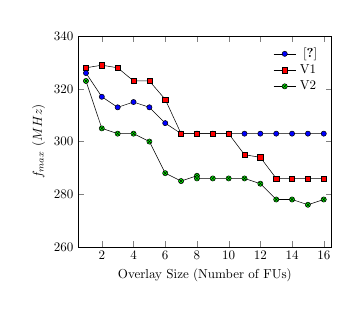
\begin{tikzpicture}[scale = 0.47]
	 \begin{axis}[
	 xlabel=Overlay Size (Number of FUs),
	 ymin=260,
	 ymax=340,
	 %ymin=200,
	 %ymax=400,
	 xmax = 16.5,
	 xmin = 0.5,
	 ylabel=$f_{max}$ ($MHz$),
	 legend pos=north east,
	 legend style={draw=none}
	 ]    

	\addplot [mark=*,mark options={fill=blue}] plot coordinates {
		(1,     326)
		(2,     317)
		(3,     313)
		(4,     315)
		(5,     313)
		(6,     307)
		(7,     303)
		(8,     303)
		(9,     303)
		(10,    303)
		(11,    303)
		(12,    303)
		(13,    303)
		(14,    303)
		(15,    303)
		(16,    303)	
	}; 
	 \addplot [mark=square*,mark options={fill=red}] plot coordinates {
	 	(1,     328)
	 	(2,     329)
	 	(3,     328)
	 	(4,     323)
	 	(5,     323)
	 	(6,     316)
	 	(7,     303)
	 	(8,     303)
	 	(8,     303)
	 	(9,     303)
	 	(10,    303)
	 	(11,    295)
	 	(12,    294)
	 	(13,    286)
	 	(14,    286)
	 	(15,    286)
	 	(16,    286)
	 }; 
	 \addplot [mark=otimes*,mark options={fill=green}] plot coordinates {
	 	(1,     323)
	 	(2,     305)
	 	(3,     303)
	 	(4,     303)
	 	(5,     300)
	 	(6,     288)
	 	(7,     285)
	 	(8,     287)
	 	(8,     286)
	 	(9,     286)
	 	(10,    286)
	 	(11,    286)
	 	(12,    284)
	 	(13,    278)
	 	(14,    278)
	 	(15,    276)
	 	(16,    278) 	
	 };

	 \legend{~\cite{li2016area}\\V1\\V2\\}
	 \end{axis}

	 \end{tikzpicture}	
	 \caption{$f_{max}$ Drop}
	 \label{fmax}
	%}
	\end{subfigure}
	
	\caption[]{V1 and V2 overlay scalability on Zynq XC7Z020.} 
	\label{scalability}
	
\end{figure}
